
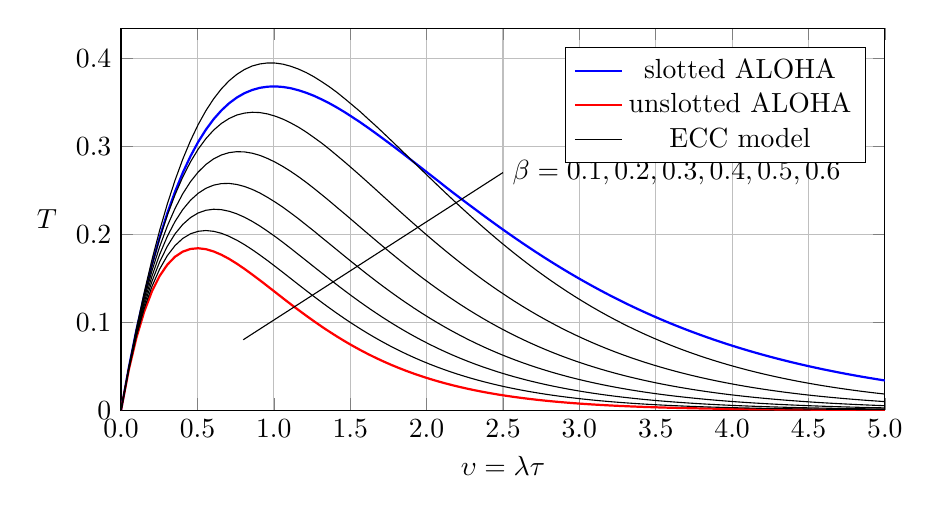
\begin{tikzpicture}[scale=1.0]

\begin{axis}
[
  title={},
  width  = 0.8*\columnwidth, 
  height = 0.4*\columnwidth,
  legend style={at={(0.975,0.95)}, anchor=north east},
%   xmode=log,
  xlabel={$\upsilon = \lambda\tau$},
  ylabel={$\mathscr{T}$}, ylabel style={rotate=-90},
%  yticklabel=\pgfmathprintnumber{\tick}\\ \%,
  xmin = 0,
  xmax = 5,
  ymin = 0,
%   ymax = 3,
  x tick label style={
        /pgf/number format/.cd,
        fixed,
        fixed zerofill,
        precision=1,
        /tikz/.cd
  },
  grid = both,
  scale only axis,
]
	\legend{slotted ALOHA, unslotted ALOHA, ECC model}
    
    \addplot[thick, blue, domain = 0:5, samples=100] {x*exp(-x)};
    \addplot[thick, red, domain = 0:5, samples=100] {x*exp(-2*x)};
    
    \foreach \a in {0.1,0.2,0.3,0.4,0.5,0.6}
        \addplot[domain = 0:5, samples=100] {x*(1+\a*x)*exp(-(2-\a)*x)};
    
    % \addplot[domain = 0.5:1.04, dashed, samples=100] {x*(1+((-3 + 2*x + sqrt(5 + 4*(-1 + x)*x))/(2*x))*x)*exp(-(2-((-3 + 2*x + sqrt(5 + 4*(-1 + x)*x))/(2*x)))*x)};
    
%     \addplot[thick] table
%     [
% 		x expr = \thisrow{lam},
%     	y expr = \thisrow{25dB}
%     ] {./Data/envelopes.dat};

    \draw[-\arrowhead] (axis cs: 0.8,0.08) -- (axis cs: 2.5,0.27) node[anchor= west] 
        {$\beta = 0.1,0.2,0.3,0.4,0.5,0.6$};
\end{axis}

\end{tikzpicture}
